\documentclass[11pt,a4paper]{article}
\usepackage[czech]{babel}
\usepackage[utf8]{inputenc}
\usepackage{amsmath}
\usepackage{float} %kvůli umístění tabulek a podobně.
%\usepackage[]{mcode} %pro matlabovský kód
\usepackage{etoolbox} %kvůli strequal v newcommand
\usepackage[czech]{babel}
\usepackage[utf8]{inputenc}

\usepackage{graphicx}	%kvůli pdf souboru z MATLABu
\usepackage{caption}		%kvůli umístění několika obrázku do jednoho figuru
\usepackage{subcaption} %kvůli umístění několika obrázku do jednoho figuru
\usepackage{setspace}	%rozteče v maticích
\usepackage{verbatim}   %víceřádkové komentáře
\usepackage{siunitx}	%hezký jednotky

\sisetup{locale = DE} % kvůli desetinné čárce (př. v siunits.)


% === Formát stránky ===
\usepackage[a4paper]{geometry}
\geometry{
	verbose,
	tmargin=2.2cm,
	bmargin=1.5cm,
	lmargin=1.5cm,
	rmargin=1.5cm}

\title{%
  Laboratorní úloha - řídící část\\
  \large Rotační kyvadlo}
\author{Tomáš Glabazňa, Matouš Vrba}
\date{\today}

\begin{document}
\maketitle

\clearpage

\section{Regulátory úhlu natočení kyvadla}
Regulátor pro kyvadlo jsme navrhovali tak, aby co nejrychleji a s co nejmenším překmitem reguloval polohu kyvadla vždy do spodní polohy, tedy na hodnotu $\varphi_p=-90^{\circ}=-\frac{\pi}{2}$. Každý regulátor jsme vždy nejdříve navrhli nějakou metodou na linearizovaném systému v pracovním bodě $\mathbf{x_0} = \left[\varphi_{m0}, \varphi_{p0}, \dot{\varphi}_{m0}, \dot{\varphi}_{p0}\right] = \left[0, -\frac{\pi}{2}, 0, 0\right]$, potom jsme ho vyzkoušeli na linearizovaném a nelineárním modelu a zkontrolovali jsme, že se chová rozumně - především jsme kontrolovali, že vstupní saturace systému nepokazí odezvy. Až pokud regulátor obstál na linearizovaném i nelineárním modelu, vyzkoušeli jsme ho na reálném systému. Zapojení pro testování regulátorů na následujícím obrázku:
\begin{figure}[H]
	\centering
    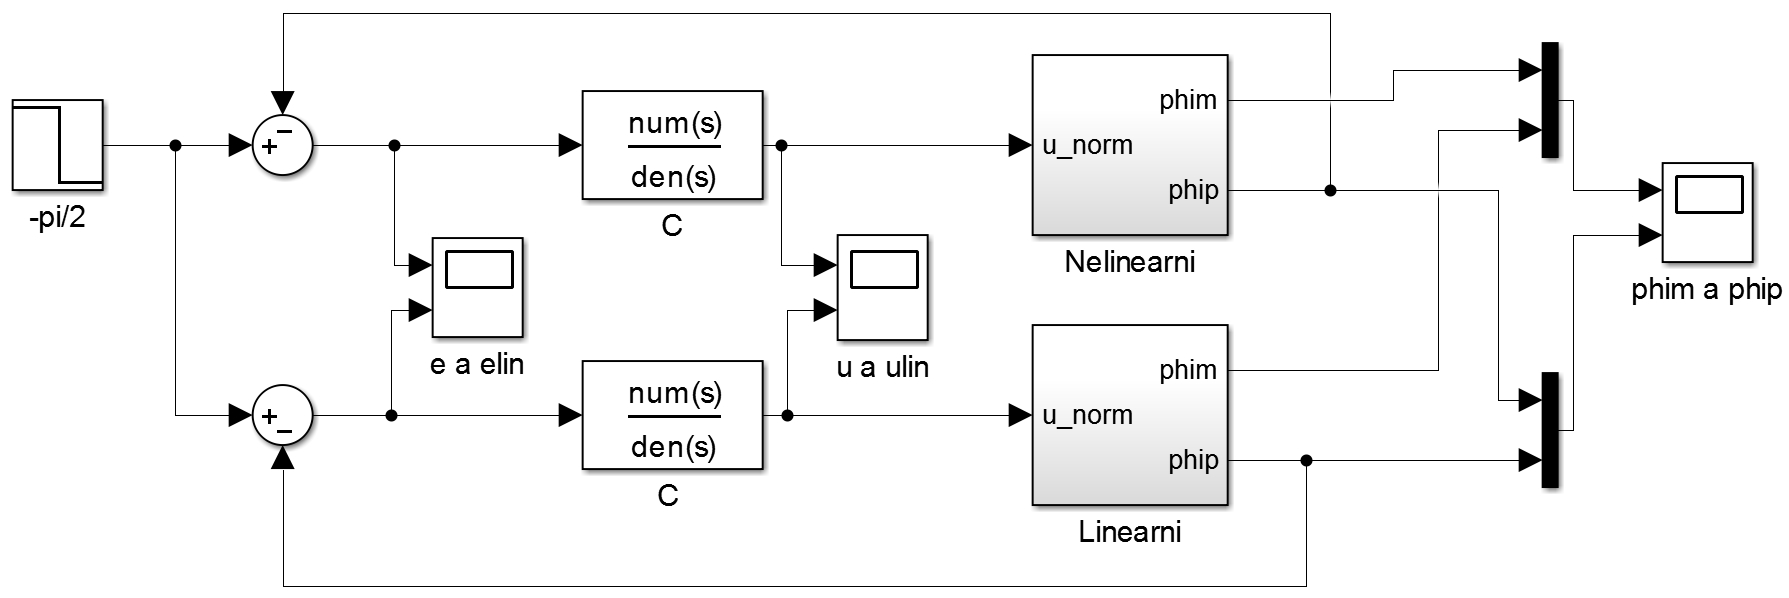
\includegraphics[scale=0.25]{schema_rizeni_nanecisto}
    \caption{Testovací zapojení regulátorů}
\end{figure}

\subsection{Obecný regulátor, navržený polynomiálními metodami}
Tento regulátor jsme navrhovali polynomiálními metodami. Nejdříve jsme si rozumně určili polohy, do kterých bychom chtěli posunout póly výsledného systému a sestavili charakteristický polynom $c(s)$ pro tyto póly. Potom jsme dosadili do rovnice pro charakteristický polynom výsledného systému se zapojeným regulátorem, kde regulátor $C = \frac{y(s)}{x(s)}$ a soustava $G = \frac{b(s)}{a(s)}$, a tuto rovnici se dvěma neznámými polynomy $y$ a $x$ vyřešili pomocí funkce Polynomial Toolboxu \textit{axbyc} s parametrem \textit{"miny"}:
\begin{align*}
c(s) &= (s + 12) (s + 5 - 10j) (s + 5 + 10j) (s + 20)^2	\\
b(s)\cdot y(s) + a(s)\cdot x(s) &= c(s)	\\
-18,1s\cdot y(s) + (s^3 + 7,021s^2 + 74,37s + 461)\cdot x(s) &=  (s + 12) (s + 5 - 10j) (s + 5 + 10j) (s + 20)^2
\end{align*}
Do žádaného charakteristického polynomu jsme museli přidat dva póly ($(s+20)^2$), aby měla tato rovnice řešení, které vede na ryzí regulátor.
\newline
Výsledný přenos regulátoru:
\begin{align*}
C = \frac{13,09s^2 - 354,3s - 1981}{16s^2 + 879,7 + 20820}
\end{align*}
Příklad odezvy kyvadla s tímto regulátorem na poruchu je na grafech na další stránce. Z grafů je vidět, že kyvadlo se neustaluje na nulové odchylce, což je způsobeno chybou enkoderových snímačů (nebo komunikace řídicího modulu s MATLABem), které někdy vynechávají kroky. Tato chyba se naintegruje a má za následek odchylku od reference, i když je kyvadlo už ve skutečnosti ustálené.
\newline
\newline
Až na tuto chybu ale regulátor funguje velmi dobře a kyvadlo stabilizuje vždy maximálně do dvou sekund.
\begin{figure}[H]
	\centering
    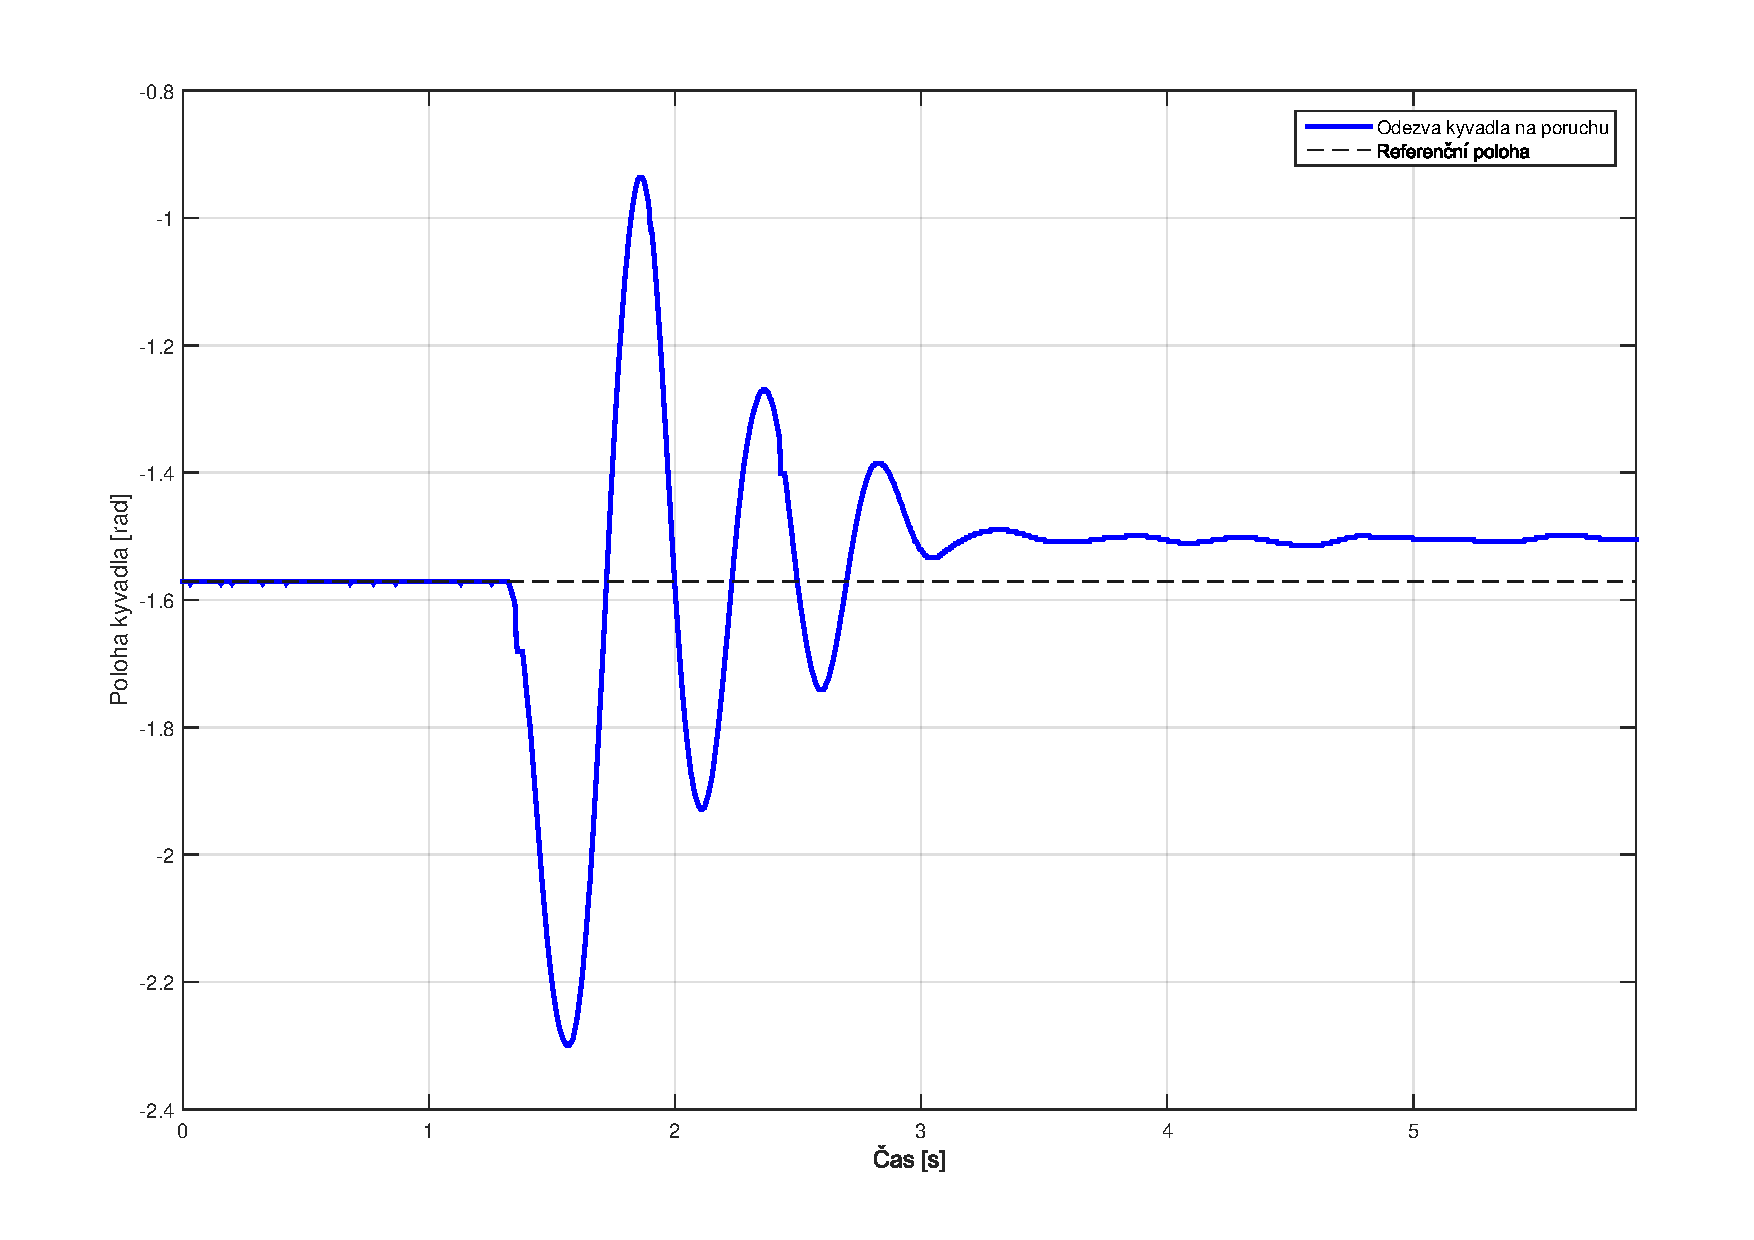
\includegraphics[scale=0.55]{odezva_kyvadlo_poly}
    \caption{Odezva kyvadla s polynomiálním regulátorem na poruchu}
\end{figure}
\begin{figure}[H]
	\centering
    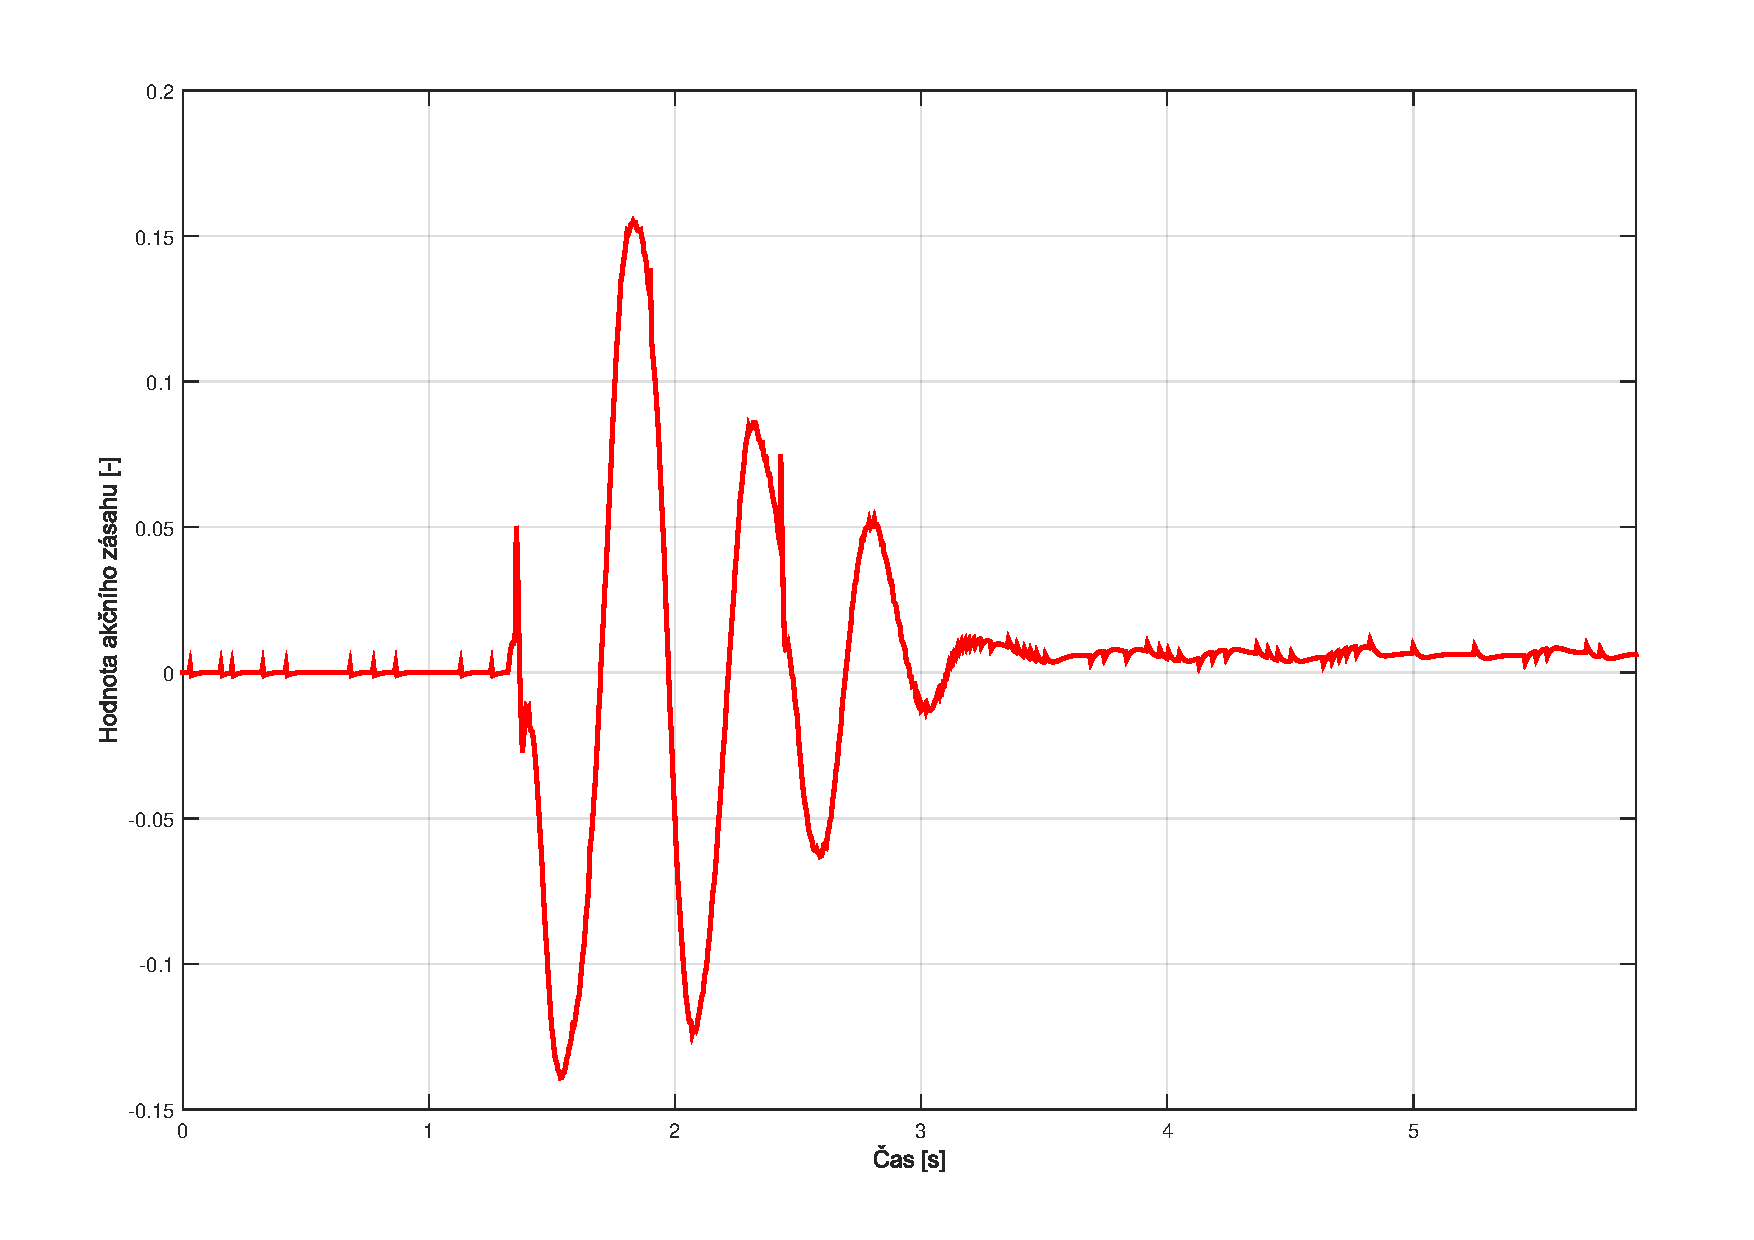
\includegraphics[scale=0.55]{odezva_kyvadlo_poly_akcnizasah}
    \caption{Akční zásah polynomiálního regulátoru}
\end{figure}


\subsection{PID regulátor, navržený autotunem}
Tento regulátor jsme navrhli po několika neúspěšných pokusech v rltoolu navrhnout nějaký rozumný PID regulátor pomocí funkce autotune. Parametry jsme nastavili na PID tuning, robustní časovou odezvu, PID s filtrovanou D složkou prvního řádu a vyváženou robustnost a výkon.
\newline
Obecná rovnice PID regulátoru a hodnoty, navržené autotunem:
\begin{align*}
C &= K_P + K_I\frac{1}{s} + K_D\frac{N}{1+N\frac{1}{s}}	\\
C &= 2,09 + 7,91\frac{1}{s} + 0,121\frac{238}{1 + 238\frac{1}{s}}
\end{align*}
Přenos, navržený autotunem:
\begin{align*}
C = -100,67\cdot\frac{(s+10,68)(s+5,715)}{s(s+238)}
\end{align*}
Následují jsou grafy odezvy kyvadla na poruchu. Tento regulátor stabilizuje velmi rychle - okolo jedné sekundy, ale kvůli nedokonalosti modelu, který nepočítá s vlivem rychlosti ramene na výchylku kyvadla, ustálenému akčnímu zásahu, který není nulový, a také kvůli již zmiňované chybě enkodérů, se systém s regulátorem po delší době destabilizuje.
\begin{figure}[H]
	\centering
    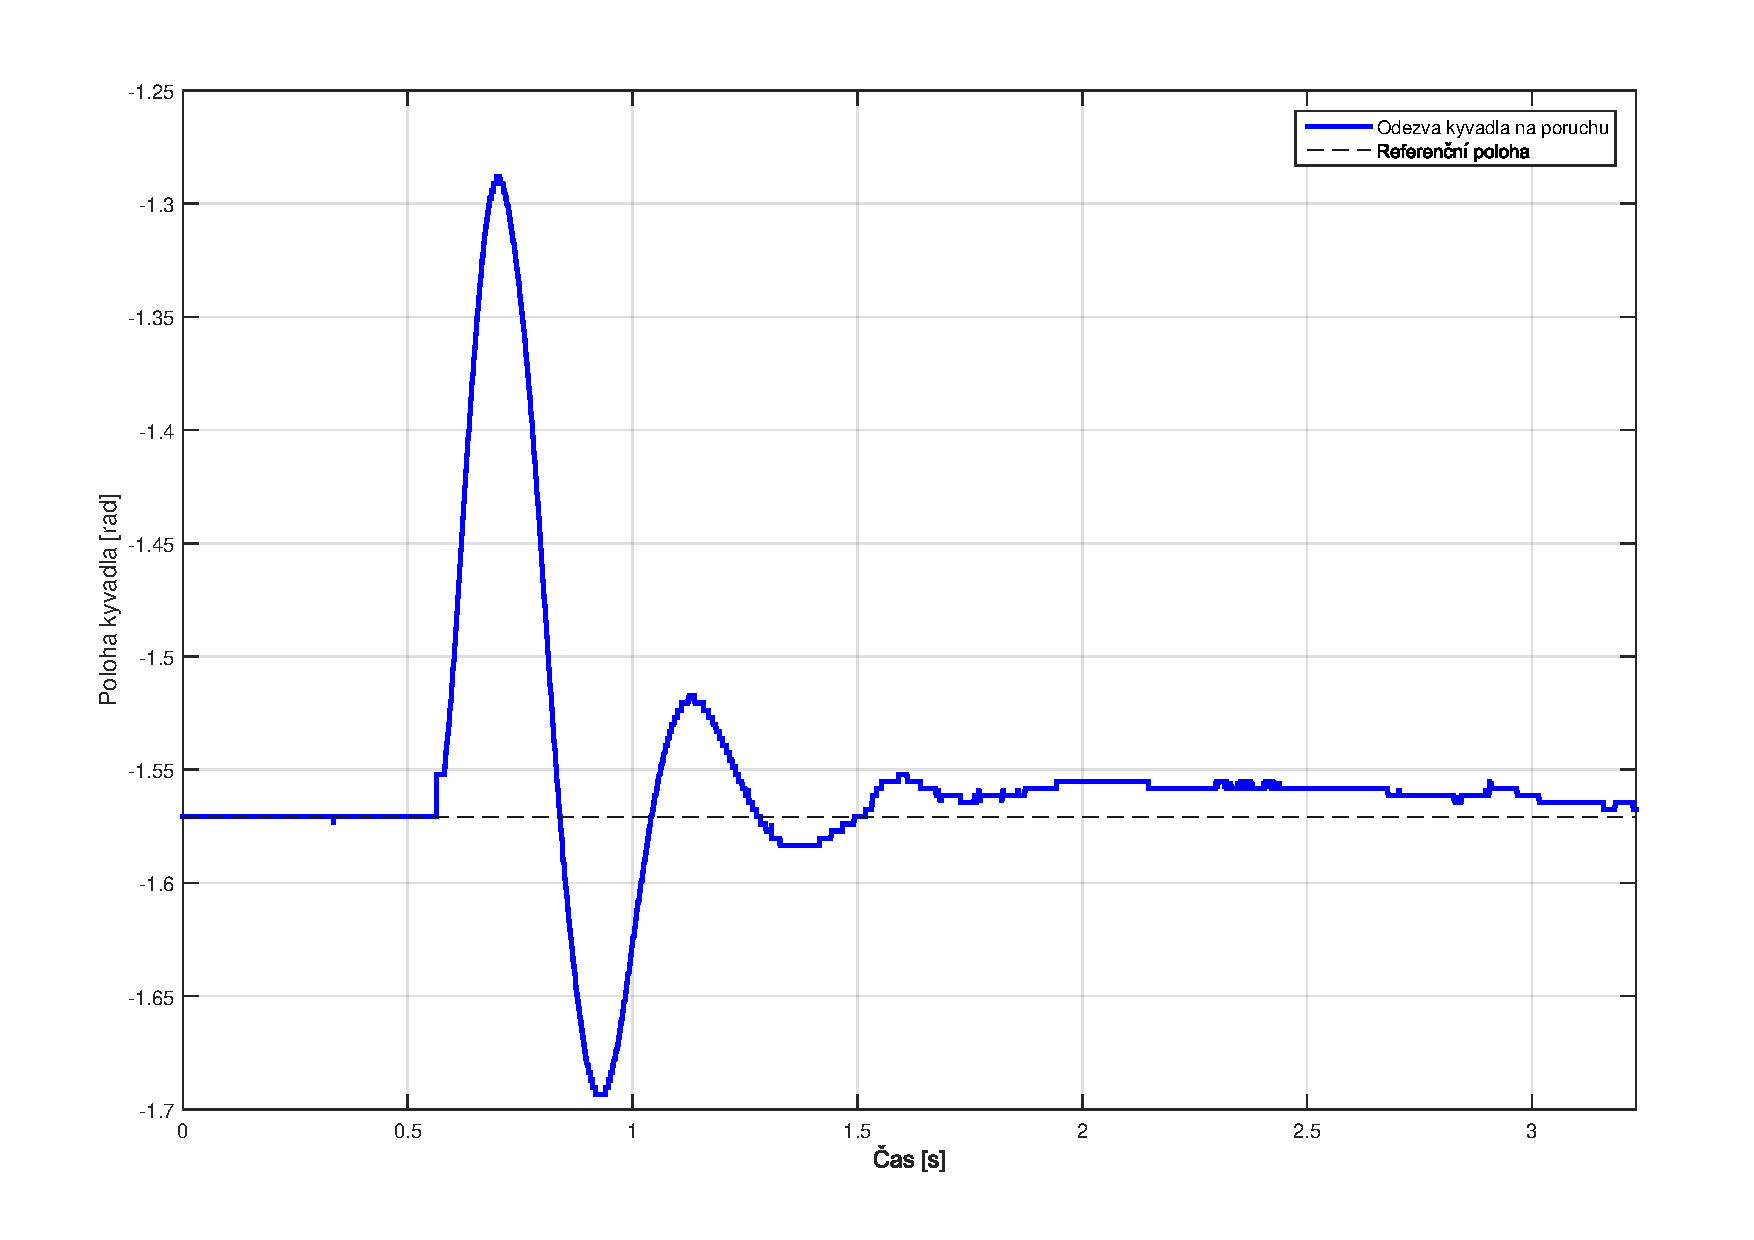
\includegraphics[scale=0.55]{odezva_kyvadlo_PID}
    \caption{Odezva kyvadla s PID regulátorem na poruchu}
\end{figure}
\begin{figure}[H]
	\centering
    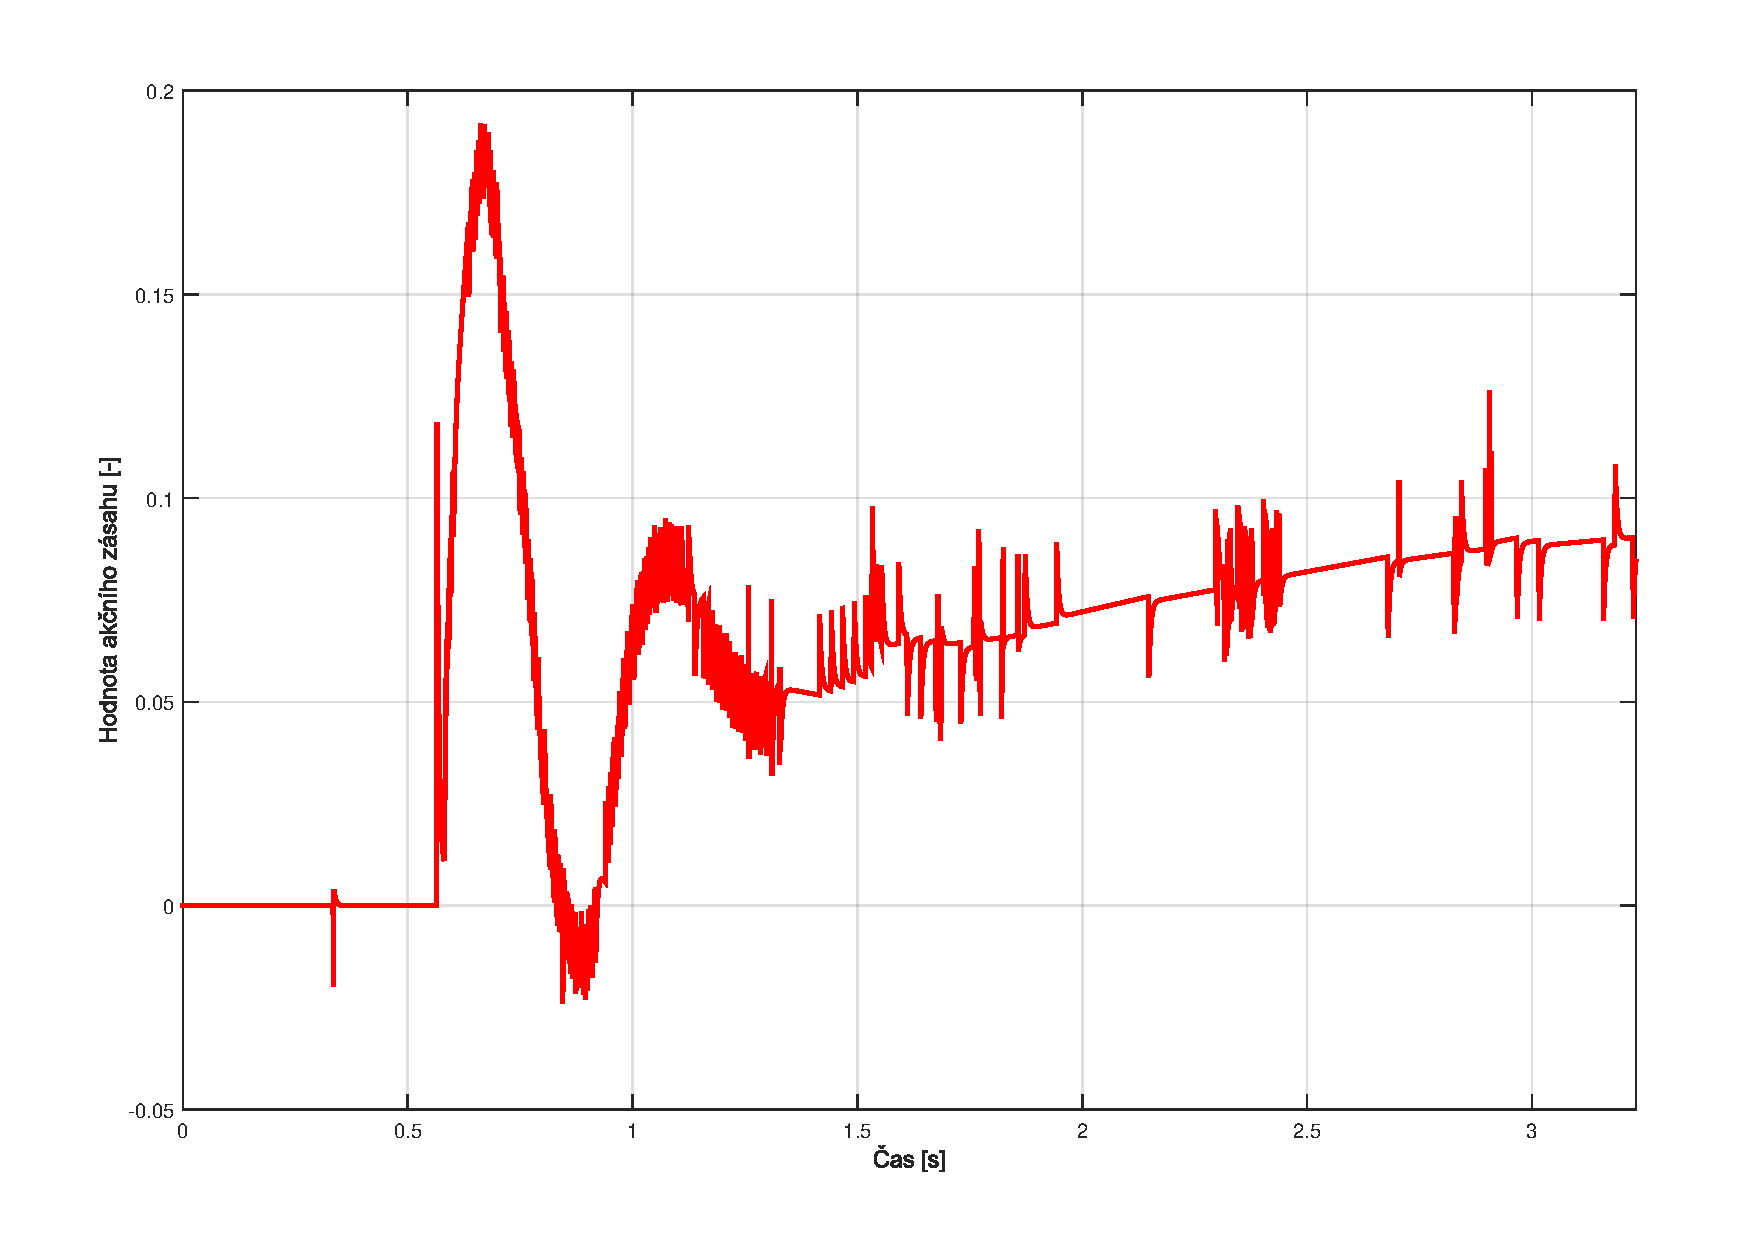
\includegraphics[scale=0.55]{odezva_kyvadlo_PID_akcnizasah}
    \caption{Akční zásah PID regulátoru}
\end{figure}


\section{Regulátory polohy ramene}
\begin{figure}[H]
\centering
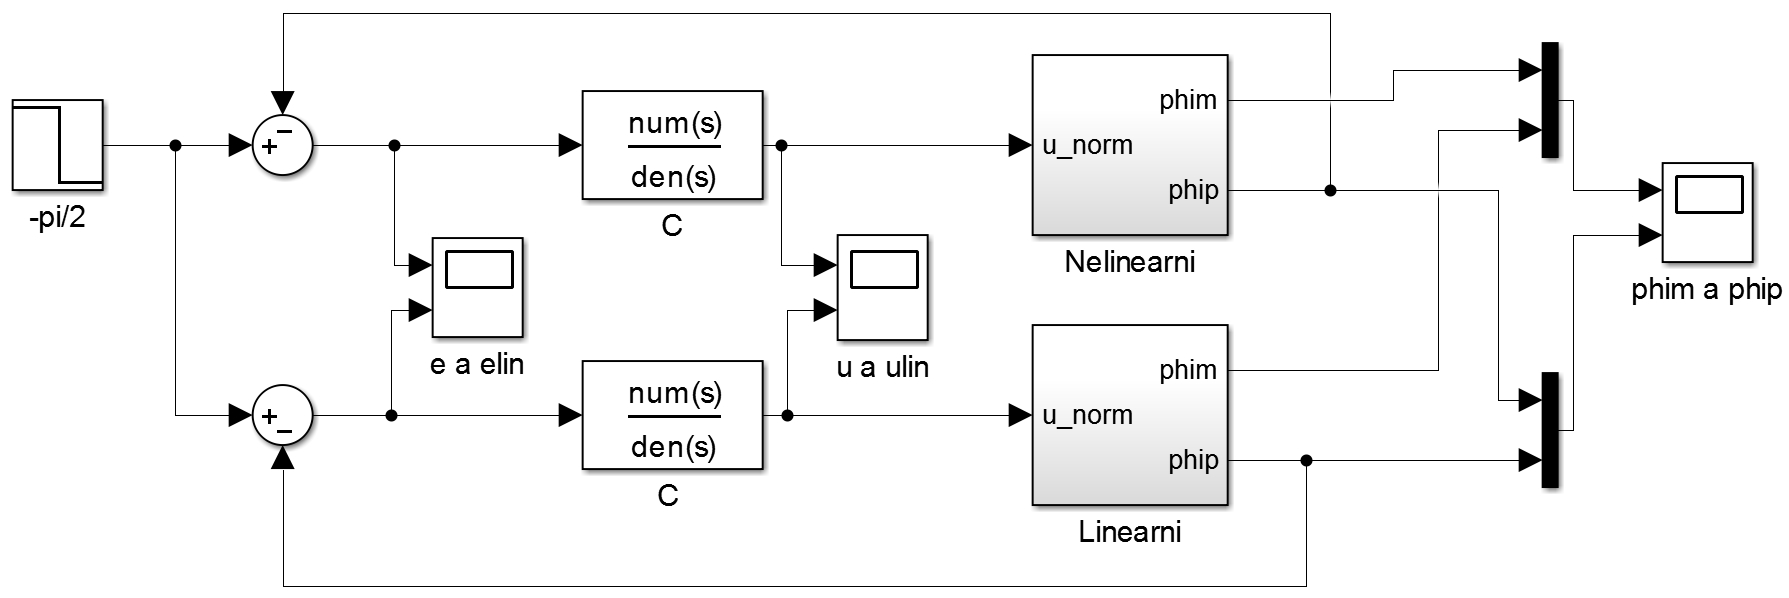
\includegraphics[width=0.7\textwidth]{schema_rizeni_nanecisto.jpg}
\caption{Zapojení pro testování regulátorů}
\label{ram_p_1}
\end{figure}

\subsection{Proporční regulátor}

Proporční zpětnovazební regulátor jsme navrhovali přímo na modelu a jeho vhodnou hodnotu jsme určili experimentálně jako 0,2. Z grafů \ref{ram_p_1} a \ref{ram_p_-1} je vidět, že překmit ramene je přibližně 10\% a rameno se ustálí v požadované hodnotě přibližně za 1 sekundu. Akční zásah, viz. graf. \ref{ram_p_akc}, sice z počátku překročí saturační hodnotu tj. 1, což však, jak jde vidět z hodnot grafu \ref{ram_p_odz}, nevadí, negativní vliv na překmit to nemá.

% P 1 
\begin{figure}[H]
\centering
\includegraphics[width=0.7\textwidth]{dobre_grafy/rameno_odezva_na1_P_akcnizasah.eps}
\caption{rameno odezva na1 P akcnizasah.eps}
\label{ram_p_1}
\end{figure}

\begin{figure}[H]
\centering
\includegraphics[width=0.7\textwidth]{dobre_grafy/rameno_odezva_na1_P.eps}
\caption{rameno odezva na1 P.eps}
\label{ram_p_1_akc}
\end{figure}
% P 1 -- end

% P -1
\begin{figure}[H]
\centering
\includegraphics[width=0.7\textwidth]{dobre_grafy/rameno_odezva_a_porucha_P_-1.eps}
\caption{rameno odezva a porucha P -1.eps}
\label{ram_p_-1}
\end{figure}

\begin{figure}[H]
\centering
\includegraphics[width=0.7\textwidth]{dobre_grafy/rameno_odezva_a_porucha_P_akcnizasah_-1.eps}
\caption{rameno odezva a porucha P akcnizasah -1.eps}
\label{ram_p_-1_akc}
\end{figure}
% P -1 -- end


\subsection{První obecný regulátor 2 řádu}
% leadlagmozna -1
\begin{figure}[H]
\centering
\includegraphics[width=0.7\textwidth]{dobre_grafy/rameno_odezva_a_porucha_leadlagmozna_-1.eps}
\caption{rameno odezva a porucha leadlagmozna -1.eps}
\label{ram_ob1}
\end{figure}

\begin{figure}[H]
\centering
\includegraphics[width=0.7\textwidth]{dobre_grafy/rameno_odezva_a_porucha_leadlagmozna_akcnizasah_-1.eps}
\caption{rameno odezva a porucha leadlagmozna akcnizasah -1.eps}
\label{ram_ob1_akc}
\end{figure}
% leadlagmozna -1 -- end

\subsection{Druhý obecný regulátor 2 řádu}

% leadlagmozna2 -1
\begin{figure}[H]
\centering
\includegraphics[width=0.7\textwidth]{dobre_grafy/rameno_odezva_a_porucha_leadlagmozna2_-1.eps}
\caption{rameno odezva a porucha leadlagmozna2 -1.eps}
\label{ram_ob2}
\end{figure}

\begin{figure}[H]
\centering
\includegraphics[width=0.7\textwidth]{dobre_grafy/rameno_odezva_a_porucha_leadlagmozna2_akcnizasah-1.eps}
\caption{rameno odezva a porucha leadlagmozna2 akcnizasah-1.eps}
\label{ram_ob2_akc}
\end{figure}
% leadlagmozna2 -1 -- end

\end{document}